% Construcción geométrica de la base recíproca (base oblicua a 60°; geometría exacta):
% g^1 es perpendicular a g2 y g^2 es perpendicular a g1, con g^i·g_i = 1 (sin suma).
% g1 = (1,0), g2 = (1/2, √3/2), g^1 = (1,−1/√3), g^2 = (0, 2/√3).
% Compilar con: scripts/compilar_tikz.sh   (→ figures/svg/base-reciproca-construccion.svg)
\def\pgfsysdriver{pgfsys-dvisvgm.def}
\documentclass[tikz,border=4pt]{standalone}
\usetikzlibrary{calc,arrows.meta,angles,quotes}
% PALETA-INICIO (generado por scripts/sincronizar_paleta.jl; no editar a mano)
\definecolor{azul}{HTML}{1B6CA8}
\definecolor{naranja}{HTML}{D95F02}
\definecolor{verde}{HTML}{2A9D8F}
\definecolor{gris}{HTML}{6B7280}
\definecolor{violeta}{HTML}{6F42C1}
\definecolor{ocre}{HTML}{8A5A00}
\definecolor{malla}{HTML}{CBD5E1}
% PALETA-FIN
\begin{document}
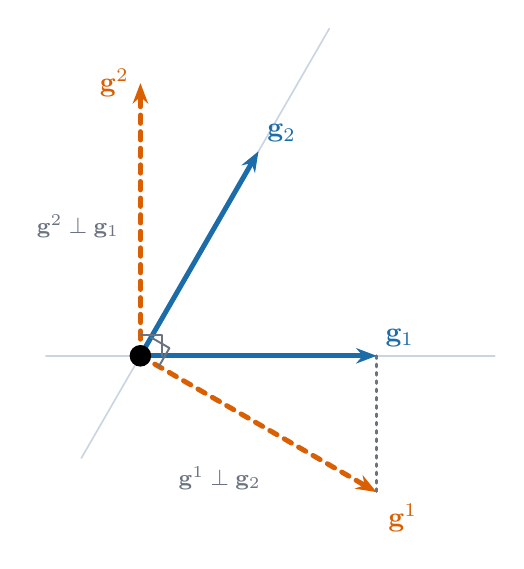
\begin{tikzpicture}[scale=3.0, line cap=round, line join=round, >={Stealth[length=2.6mm]}]
  \pgfmathsetmacro{\rt}{sqrt(3)}
  \coordinate (O) at (0,0);
  \coordinate (G1) at (1,0);
  \coordinate (G2) at (0.5,{\rt/2});
  \coordinate (R1) at (1,{-1/\rt});
  \coordinate (R2) at (0,{2/\rt});
  % rectas a las que son perpendiculares
  \draw[malla, line width=0.6pt] ($(O)!-0.5!(G2)$) -- ($(O)!1.6!(G2)$);
  \draw[malla, line width=0.6pt] (-0.4,0) -- (1.5,0);
  % g^1 ⟂ g2 : pie de la proyección de g1 sobre la normal a g2 y plano de g1·g^1 = 1
  \draw[gris, dotted, line width=1pt] (G1) -- (R1);
  \draw[naranja, ->, dashed, line width=1.8pt] (O) -- (R1) node[below right] {$\mathbf{g}^1$};
  \draw[naranja, ->, dashed, line width=1.8pt] (O) -- (R2) node[left] {$\mathbf{g}^2$};
  \draw[azul, ->, line width=1.8pt] (O) -- (G1) node[above right=-1pt] {$\mathbf{g}_1$};
  \draw[azul, ->, line width=1.8pt] (O) -- (G2) node[above right=-1pt] {$\mathbf{g}_2$};
  % ángulos rectos: g^1 ⟂ g2 (en la dirección −30° y 60°) y g^2 ⟂ g1
  \draw[gris, line width=0.7pt] (-30:0.09) -- ($(-30:0.09)+(60:0.09)$) -- (60:0.09);
  \draw[gris, line width=0.7pt] (0.09,0) -- (0.09,0.09) -- (0,0.09);
  \node[font=\footnotesize, gris, anchor=east] at (0.55,-0.52) {$\mathbf{g}^1\perp\mathbf{g}_2$};
  \node[font=\footnotesize, gris, anchor=east] at (-0.05,0.55) {$\mathbf{g}^2\perp\mathbf{g}_1$};
  \fill (O) circle (1.3pt);
\end{tikzpicture}
\end{document}
